Das Elektronenmikroskop ist eine spezielle Art von Mikroskop, das Elektronen anstelle von Licht verwendet, um eine stark vergrößerte und hochauflösende Abbildung der Probe zu erzeugen. 
Im Vergleich zum Lichtmikroskop bietet es eine wesentlich höhere Vergrößerung sowie eine deutlich präzisere Bilddarstellung.

Einige Elektronenmikroskope ermöglichen eine Vergrößerung von bis zu zwei Millionen Mal der tatsächlichen Größe des Objekts, während selbst die leistungsfähigsten Lichtmikroskope auf etwa 2000-fache Vergrößerung begrenzt sind. Sowohl im Licht- als auch im Elektronenmikroskop gibt es jedoch durch die jeweilige Wellenlänge physikalisch bedingte Grenzen hinsichtlich der Auflösung und Bildschärfe.

Die überlegene Auflösung und Vergrößerungsfähigkeit des Elektronenmikroskops ist auf die deutlich kürzere Wellenlänge der Elektronen zurückzuführen – gemäß der de-Broglie-Gleichung – im Vergleich zur Wellenlänge elektromagnetischer Strahlung (Licht). Daraus ergibt sich ein inverser Zusammenhang zwischen Wellenlänge und Auflösung bzw. 
Vergrößerung: Je kürzer die Wellenlänge, desto höher die mögliche Auflösung.

 \newpage
\vspace{0.2cm}
\begin{figure}
    \centering
    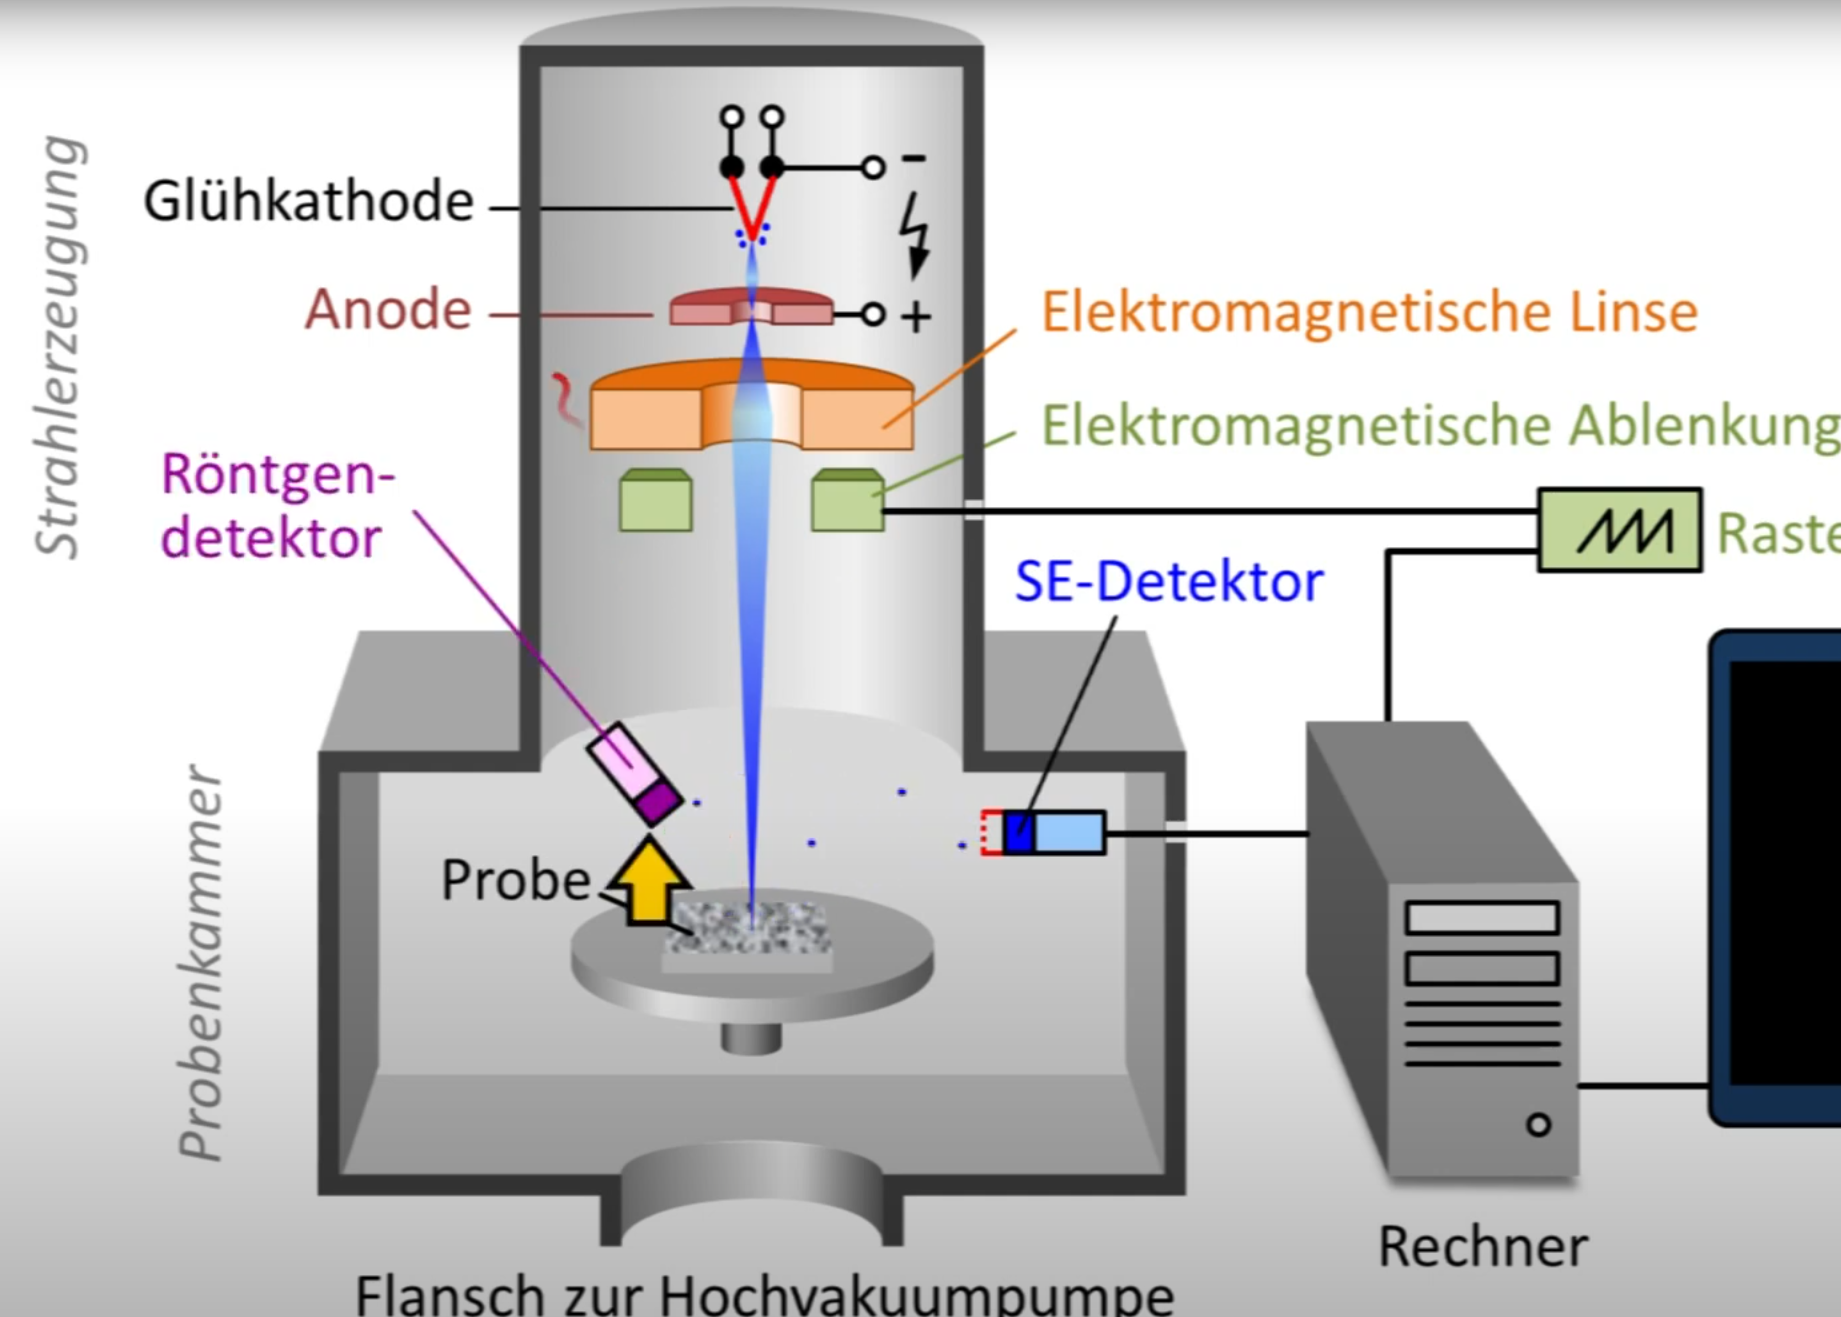
\includegraphics[scale=0.3]{Bilder/Screenshot 2025-04-10 165235}
    \caption{Erklärung zur Elektronenstrahlerzeugung im REM}
    \par Quelle: \href{https://www.youtube.com/watch?v=uXjXx63Nb6k&t=286s}{Youtube: Das Rasterelektronenmikroskop}
    \vspace{0.2cm}
    \label{Abb.1: Erklärung zur Elektronenstrahlerzeugung im REM }
\end{figure} 
\vspace{0.2cm}
Die Kathode wird stark erhitzt, auf etwa 1800K. Zusätzlich wird eine Hochspannung von etwa 5 bis 15kV zwischen Kathode und Anode angelegt. 
Dadurch erhalten die Elektronen genügend Energie, um beschleunigt zu werden. So entsteht ein Elektronenstrahl, der jedoch erst durch elektromagnetische Linsen gebündelt und fokussiert werden kann.
\\ \\
Mithilfe elektromagnetischer Ablenkung kann der gebündelte Strahl über die Probe geführt werden, sodass unterschiedliche Positionen gezielt angesteuert werden können. 
Zur Detektion der Elektronen wird ein positiv geladener Sekundärelektronendetektor verwendet, der die negativ geladenen Elektronen anzieht. Diese werden anschließend mithilfe einer Computersoftware visuell dargestellt.
\\
Beim Betrieb des Rasterelektronenmikroskops entsteht außerdem Röntgenstrahlung.\cite{key1} 
Diese kann mit einem Röntgendetektor erfasst werden, um die chemische Zusammensetzung des untersuchten Materials zu bestimmen.